\documentclass[lualatex, article]{jlreq}

% Packages
\usepackage{luatexja}     % Japanize
\usepackage[backend=biber,
            style=alphabetic,
            sorting=none,
            ]{biblatex}    % bibliography
\usepackage{amsthm}        % proof environment
\usepackage{algorithmic}   % algorithmic environment
\usepackage{algorithm}     % algorithm environment

\addbibresource{references.bib}

% Japanize
\newtheorem{theorem}{定理}
\newtheorem{lemma}{補題}
\newtheorem{definition}{定義}
\newtheorem{corollary}{系}

% Metadata
\title{7.8 施設配置問題に対する局所探索アルゴリズム}
% \subtitle{近似アルゴリズム ―離散最適化問題への効果的アプローチ―}
\author{岡山 大輝}
% \institute{兵庫県立大学大学院 情報科学研究科\textit{(ad25r010@guh.u-hyogo.ac.jp)}}
\date{January 5 2026 \& January 12, 2026}


\begin{document}

\maketitle{}

\section*{記法／変数のまとめ}

\begin{enumerate}
  \leftskip 2em

  \item[\(F\): ] 施設集合, Facility set
  \item[\(D\): ] 利用者集合, Demand set
  \item[\(f_i\): ] 施設 \(i\) の開設コスト
  \item[\(c(i,j)\): ] 施設 \(i\) と利用者 \(j\) 間の距離
  \item[\(S (\subseteq F)\): ] 開設する施設
  \item[\(\sigma: D \to S\): ] 利用者から施設への割当関数
\end{enumerate}

\begin{figure}
  \centering
  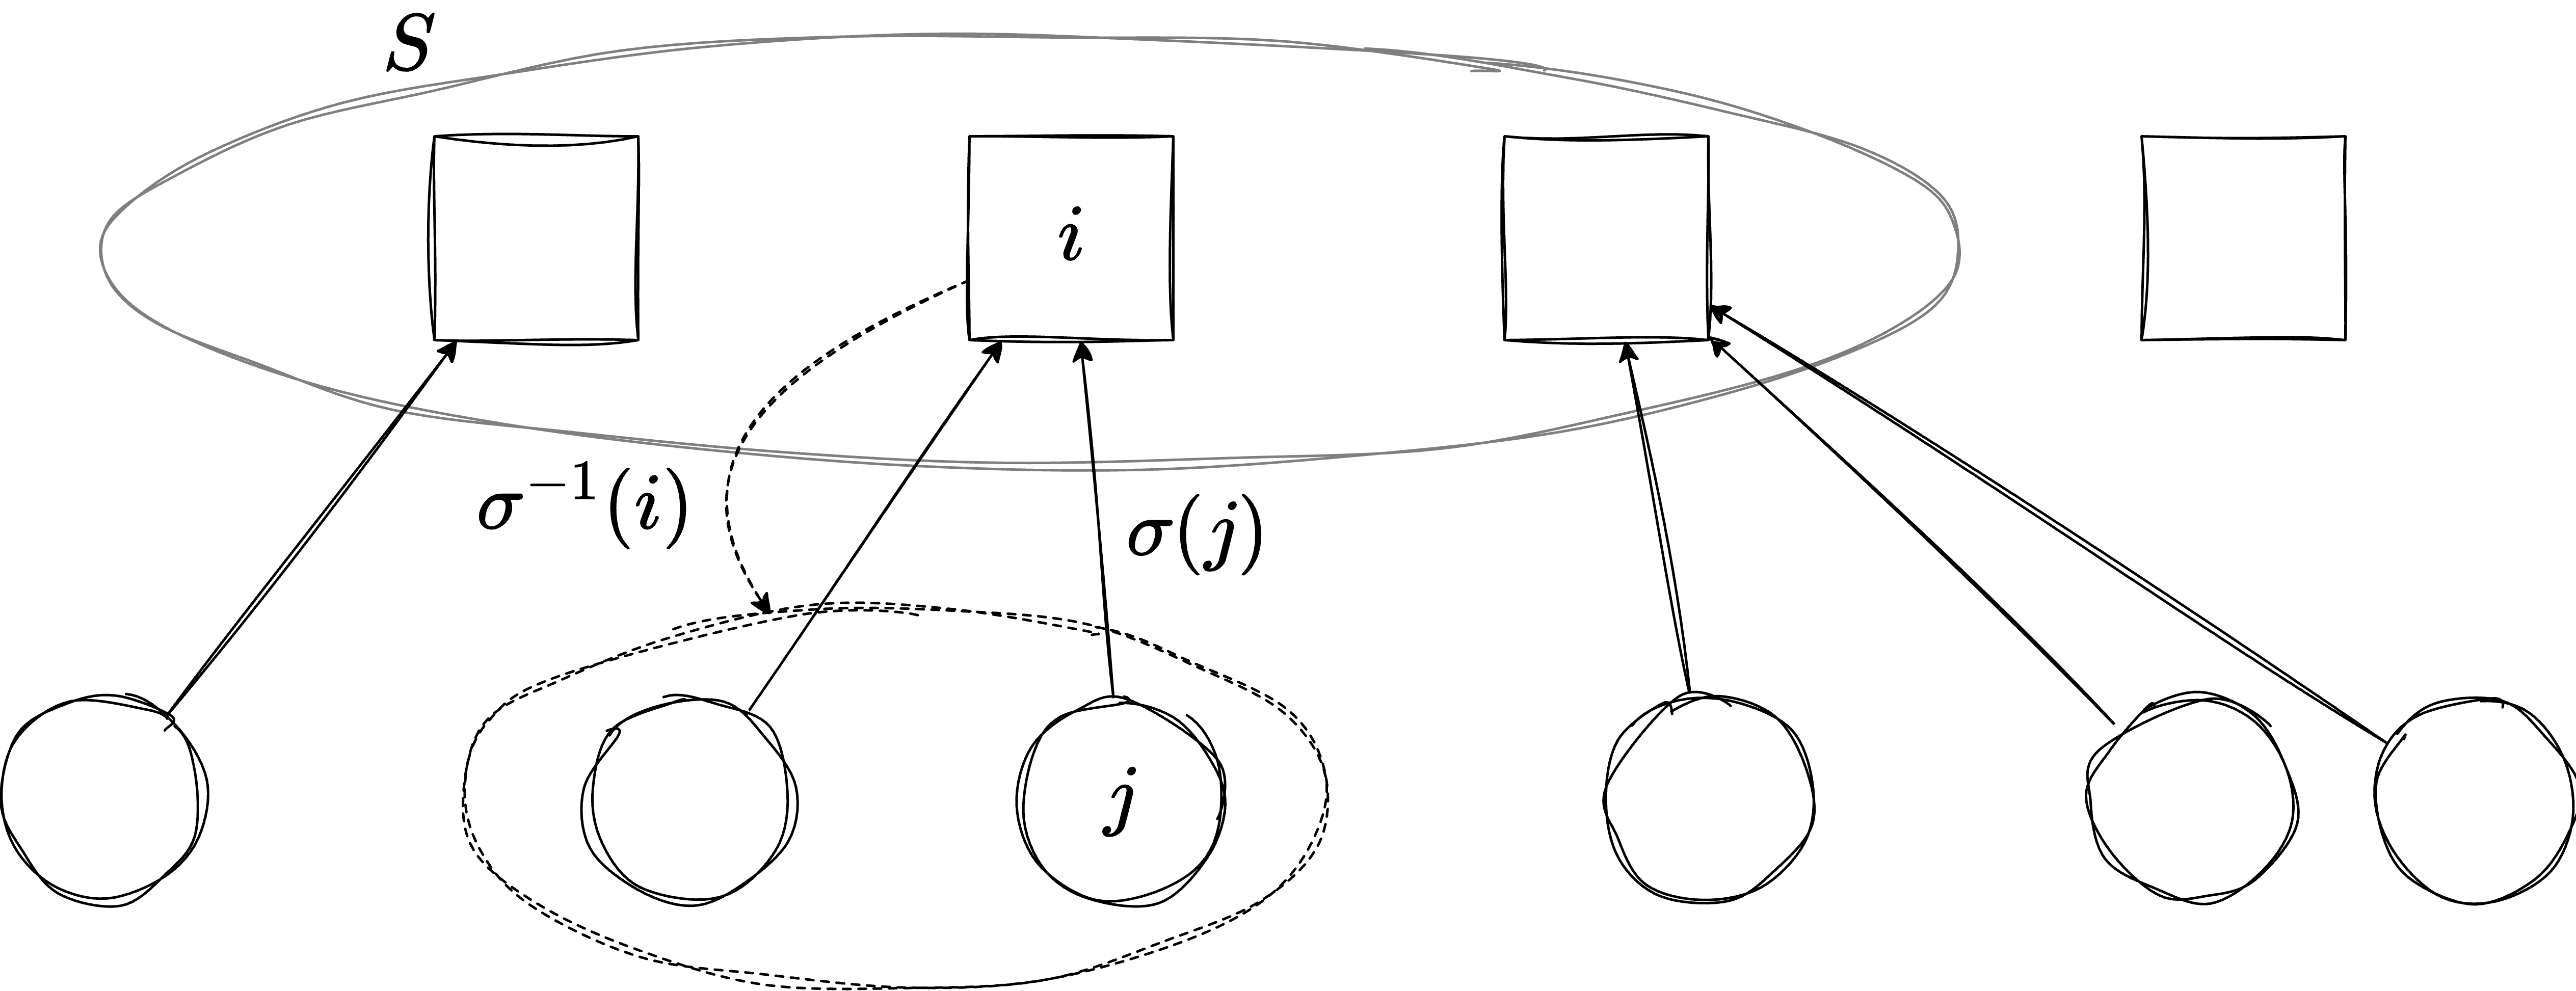
\includegraphics[width=0.7\textwidth]{figures/notations.drawio.png}
  \caption{施設配置問題における記法のまとめ}
\end{figure}

\printbibliography[title=引用文献]{}


\end{document}
